\chapter{Surfaces de Riemann}
\section{Un exemple: la racine carrée}
Soit à calculer l'intégrale suivante:
\[
I = \int_{\mathcal{C}(0,1)} \frac{dz}{2 \sqrt{z}}
\]
où $\mathcal{C}(0,1)$ est le cercle unité parcouru une seule fois en sens trigonométrique. La formule donnant l'intégrale d'une application continue le long d'un chemin de classe $C^1$ donne:
\[
I = \frac{1}{2} \int_0^{2\pi} i e^{it}e^{-it/2} dt = \frac{i}{2} \int_0^{2\pi} e^{it/2} dt= -2
\]
Si l'on parcourt maintenant deux fois le même contour, l'application de la même formule conduit à un résultat pour le moins surprenant:
\[
\frac{i}{2} \int_{0}^{4 \pi} e^{it/2} dt= 0 \neq 2 I 
\]
Que s'est-il donc passé ? Une clé de compréhension de ce phénomène est donnée par la proposition suivante:
\begin{prop}
Il n'existe pas d'application continue $f \colon \C \to \C$ telle que $f^2(z) = z$.
\end{prop}
\begin{proof}
Soit $f$ vérifiant pour tout $z\in \C$: $f^2(z)=z$. En écrivant $z$ sous forme polaire, il vient:
\[
f^2\left(r e^{it}\right) = r e^{it}
\]
soit encore:
\[
f\left(r e^{it}\right) = \sqrt{r} e^{it/2} \text{ (détermination positive)}
\]
ou:
\[
f\left(r e^{it}\right) = - \sqrt{r} e^{it/2} \text{ (détermination négative)}
\]
Soit $\gamma \colon t \in [0,2\pi] \mapsto e^{it}$ un paramétrage du cercle unité. On a $f\circ \gamma(0^+)= 1 (\text{resp.} -1) \neq f\circ \gamma(2 \pi^-)= f \circ \gamma(2\pi^-)=-1(\text{resp.} 1)$, prouvant ainsi que $f$ ne peut être continue.
\end{proof}
Un problème similaire avait été rencontré dans le cas du logarithme complexe et se résout classiquement par l'introduction d'une coupure. Dans le cas de la racine carrée, on choisit généralement de supprimer l'axe réel négatif pour conserver la définition usuelle, mais il n'existe que deux déterminations (alors qu'il en existe une infinité pour le log) :
\[
\begin{cases}
&\sqrt{r e^{it}}_+ = \sqrt{r} e^{it/2} \\
&\sqrt{r e^{it}}_- = -\sqrt{r} e^{it/2}
\end{cases}
\]
Cela interdit néanmoins le contour d'intégration $\mathcal{C}(0,1)$, que l'on peut cependant voir comme une intégrale généralisée, avec le paramétrage $\gamma \colon t \in ]-\pi,\pi[ \to e^{it}$:
\[
\frac{i}{2} \int_{-\pi^+}^{\pi^-} e^{it/2} dt = 2i
\]
Le résultat obtenu est différent de celui obtenu pour $I$, ce qui n'est guère satisfaisant. Toute la difficulté réside dans le fait que l'application "racine carrée" n'est pas correctement définie sur $\C$, tout comme d'ailleurs sur $\R$. Si l'on cherche en effet à résoudre l'équation $w^2 = z$ avec $(z,w)\in \C$, on obtient non pas le graphe d'une fonction, mais une surface de $\C^2$, formée des couples $(z=r e^{it},w=\pm \sqrt{r} e^{it/2})$. L'image \ref{fig:sqrt_} correspond à la partie réelle de la coordonnée $w$ de cette surface.
%\footnote{Crédit:  Wlongqi - Own work, CC BY-SA 3.0, \url{https://commons.wikimedia.org/w/index.php?curid=5964270}}

%\begin{figure}[h]
%	\centering
%	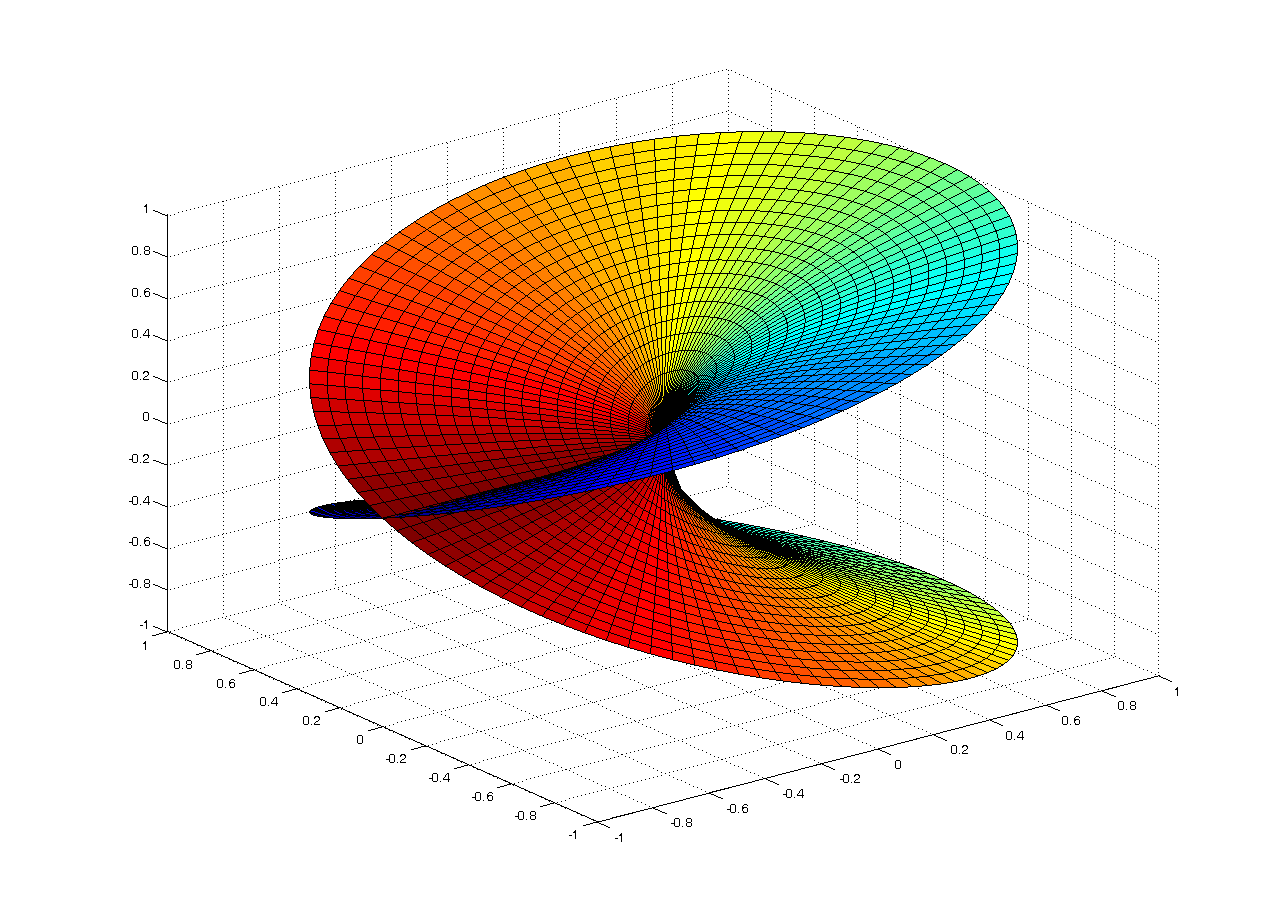
\includegraphics[scale=0.3]{Riemann_sqrt.png}
%	\caption{Partie réelle de la surface $w^2=z$}
%\end{figure}

\begin{figure}[hbt]
\begin{center}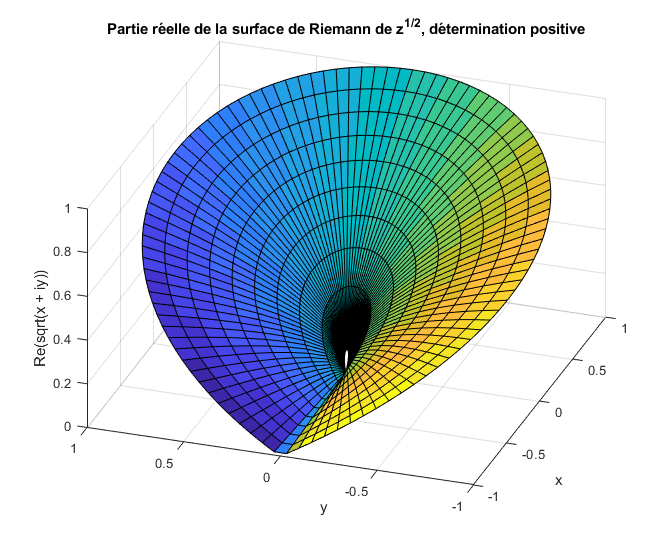
\includegraphics[scale=0.46]{images/Surf_Riema_sqrt_Re_positive.PNG}
\end{center}
\caption{Partie réelle de la surface $w^2=z$, détermination positive}\label{fig:sqrt_positive}
\end{figure}

\begin{figure}[hbt]
\begin{center}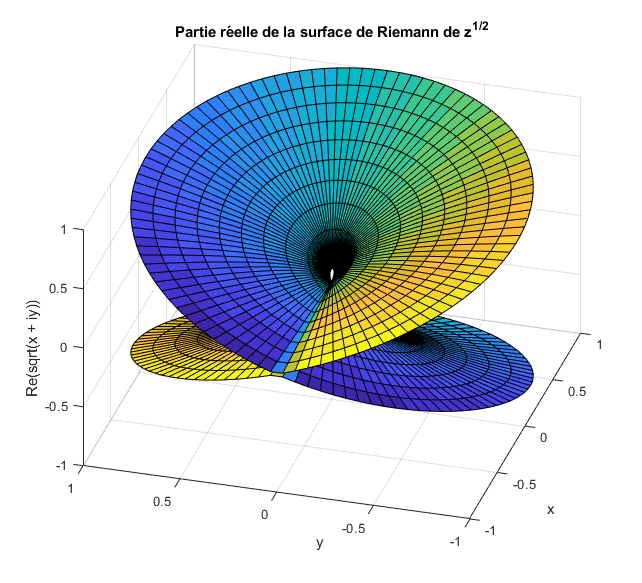
\includegraphics[scale=0.46]{images/Surf_Riema_sqrt_Re.PNG}
\end{center}
\caption{Partie réelle de la surface $w^2=z$}\label{fig:sqrt_}
\end{figure}

L'idée (due à B. Riemann) qui va maintenant être formalisée, consiste à remplacer l'intégration dans $\C$ par une intégration dans $\C^2$ en se restreignant à la surface de Riemann.
\section{Surfaces de Riemann abstraites}
Une surface de Riemann définie de façon générale est une abstraction de la notion de surface concrète dans $\C^2$. Dans la plupart des cas, il sera cependant possible d'en obtenir une image locale sous la forme d'un graphe de fonction. Le point de départ de la théorie est la proposition suivante.
\begin{prop}
	\label{prop:chg_var}
	Soit $\Omega$ un domaine de $\C$ et soit $\phi \colon \Omega ( \subseteq \C) \to \phi(\Omega) (\subseteq \C)$ une bijection holomorphe ainsi que son application réciproque. Pour tout chemin $\gamma \colon [a,b] \to \Omega$ et toute application continue $f \colon \phi(\Omega) \to \C$, on a:
	\[
	\int_{\phi \circ \gamma} f(z)dz = \int_\gamma f \circ \phi(z) \phi^\prime(z)dz
	\]
\end{prop}
\begin{proof}
	Il s'agit d'une application directe du théorème des fonctions composées. On a:
	\[
	\int_{\phi \circ \gamma} f(z)dz = \int_a^b f\left(\phi \circ \gamma(t)\right)\phi^\prime(\gamma(t)) \gamma^\prime(t) dt = \int_\gamma f \circ \phi(z) \phi^\prime(z)dz
	\]
\end{proof}
A partir de ce résultat, on remarque qu'une intégrale de chemin peut se définir soit sur le domaine, soit sur l'image du domaine par un difféomorphisme de $\C$.
\begin{fdefn}
	Une surface de Riemann est un espace topologique connexe $X$ pour lequel il existe une famille d'ouverts $(U_i)_{i \in I}$ recouvrant $X$ et des homéomorphismes $(\phi_i)_{i \in I} \colon U_i \to V_i$ avec $(V_i)_{i \in I}$ ouverts de $\C$ telles que les applications:
	\begin{align*}
	    \psi_i^j \colon \phi_i (U_j\cap U_i) & \longrightarrow  \phi_j (U_i\cap U_j), \,  \forall(i,j) \in I^2, \\
	    z  & \longmapsto \phi_j\circ \phi_i^{-1}(z)
	\end{align*}
	soient holomorphes ainsi que leurs applications réciproques (on dit encore qu'elle sont biholomorphes).
\end{fdefn}
\begin{defn}
Les applications  $\phi_i$ définies ci-dessus sont les \textbf{cartes locales} de $X$, les applications $\psi_i^j$ définies ci-dessus sont les applications de changement de carte.
\end{defn}
\begin{exem}
Soit $\Omega \subset \C$ un domaine. C'est une surface de Riemann avec l'unique carte locale $\phi \colon z \in \Omega \mapsto z$ ($\phi$ est donc l'application identité).
\end{exem}
\begin{exem}
La sphère de Riemann $\overline{\C}$ offre un exemple non trivial de surface de Riemann. Deux cartes locales sont nécessaires:
\[
    \phi_1 \colon z \in \overline{\C} \setminus \{\omega\} \mapsto z \in \C
\]
et
\[
\phi_2 \colon z \in \overline{\C} \setminus \{0\} \mapsto 1/z
\]
avec la convention $1/\omega=0$ assurant la continuité. Les applications de changement de carte sont:
\[
\psi_1^2 =\psi_2^1 \colon z \in \overline{\C} \setminus \{\omega,0\} \mapsto 1/z
\]
qui sont holomorphes sur leur domaine de définition.
\end{exem}
\begin{defn}
	Soit $X$ une surface de Riemann et $\Omega$ un ouvert de $X$. On dira que $f \colon \Omega \to \C$ est continue (resp. holomorphe) si pour tout $i \in I$, $f \circ \phi_i^{-1}$ est continue (resp. holomorphe) sur $\phi_i(U_i \cap \Omega)$.
\end{defn}
On notera que l'on peut définir une application continue (resp. holomorphe) sur $X$ en considérant une famille $f_i \colon V_i \to \C, i \in I$ vérifiant pour tout couple $(i,j)\in I^2$:
\[
\forall z \in \phi_i(U_i \cap \Omega), f_i(z) = f_j \circ \psi_i^j(z)
\]
Il suffit alors de poser $f(z)=f_i \circ \phi_i(z), z \in \Omega \cap U_i$.
\begin{defn}
Soient $X,Y$ deux surfaces de Riemann et $f \colon X \to Y$. On dira que $f$ est continue (resp. holomorphe) si pour tout couple de cartes locales $\phi_i \colon U_i \to \phi(U_i), \phi_j \colon W_j \to \phi(W_j)$, l'application $\phi_j \circ f \circ \phi_i^{-1}$ est continue (resp. holomorphe).
\end{defn}
\begin{rem}
On peut étendre immédiatement cette définition au cas où l'application $f$ est définie seulement sur un ouvert de $X$.
\end{rem}
\begin{prop}
Les applications holomorphes $f \colon \Omega \to \overline{\C}$, avec $\Omega$ ouvert de $\C$ sont les applications holomorphes de $\Omega \to \C$ ou les applications n'admettant que des pôles comme points singuliers. 
\end{prop}
\begin{proof}
    Il est clair que si $f$ est holomorphe de $\C$ dans $\C$, alors elle est holomorphe dans $\overline{\C}$. Sinon, il existe des points où $f$ est non bornée. Au voisinage de l'un ces points, noté $z_0$, l'application lue dans la carte $\phi_2$ est $1/f$ et par continuité on aura $1/f(z_0) = 0$. Comme $1/f$ est holomorphe et n'est pas identiquement nulle, elle s'exprime sous la forme $1/f(z_0) = (z-z_0)^p g(z)$ avec $g$ ne s'annulant pas dans un voisinage de $z_0$. On en déduit immédiatement que $z_0$ est un pôle d'ordre au plus $p$ de $f$. 
\end{proof}
\begin{rem}
Les applications holomorphes de $\C$  dans $\overline{\C}$ sont appelées applications méromorphes.
\end{rem}
\begin{prop}
\label{prop:surface_racine}
L'ensemble $\mathcal{S}$ des couples $(z,w) \in \C^2$ tels que $w^2=z$ est une surface de Riemann.
\end{prop}
\begin{proof}
La topologie induite sur $\mathcal{S}$ est celle pour laquelle une partie $U$ de $\mathcal{S}$ est ouverte si et seulement si elle est l'intersection d'un ouvert de $\C^2$ avec $\mathcal{S}$. On va considérer trois ouverts et les cartes locales associées:
\[
\left \{
%\begin{cases}
\begin{array}{r c l}
\phi_1 \colon  U_1 = \{ (z,w)\in \mathcal{S}\, | \, \Re \text{e}(w) > 0 \}  &\to&  \C \setminus \R^-\\
 (z, w)  &\mapsto&  z \\
\phi_2 \colon  U_2 = \{ (z,w)\in \mathcal{S}\, | \, \Re \text{e}(w) < 0 \} &\to& \C \setminus \R^-\\
 (z, w)  &\mapsto&  z \\
\phi_3 \colon U_3 = \{ (z,w)\in \mathcal{S}\, | \, \Re \text{e}(w) \in ]-2,2[ \} &\to& ]-2,2[ + i \R \\
 (z, w)  &\mapsto&  w \\ 
\end{array}
\right .
%\end{cases}
\]
Les deux applications de changement de carte à considérer sont $\psi_3^1 = \phi_1 \circ \phi_3^{-1}$ et $\psi_3^2 = \phi_2 \circ \phi_3^{-1}$ vérifiant:
\[
\begin{cases}
\begin{array}{rccl}
\psi_3^1 \colon & ]0,2[ + i \R & \longrightarrow  \C \\
& w & \longmapsto  w^2 \\
\psi_3^2 \colon & ]-2,0[ + i \R & \longrightarrow  \C \\
& w & \longmapsto  w^2    
\end{array}

\end{cases}
\]
Leurs domaines respectifs excluant l'axe imaginaire, il s'agit bien d'applications biholomorphes. 
\end{proof}
\begin{defn}
\label{def:forme_degre_un}
Soit $X$ une surface de Riemann dont la famille des cartes locales est $(U_i,\phi_i)_{i \in I}$. Une forme différentielle $f$ de degré un sur un ouvert $\Omega \subset X$ est la donnée d'une famille d'applications continues $f_i \colon \phi_i(U_i \cap \Omega) \to \C, i \in I$ vérifiant la condition:
\[
\forall (i,j)\in I^2, \forall z \in \phi_i\left(U_i\cap U_j \cap \Omega\right), f_j\left(\psi_i^j(z)\right)\left(\partial_z \psi_i^j(z)\right)=f_i(z)
\]
\end{defn}
\begin{rem}
On notera dans la suite $f_i dz$ la forme différentielle dans l'ouvert $\phi_i(U_i\cap \Omega)$. Cette notation est cohérente avec la notion d'intégrale le long d'un chemin qui sera l'objet de la définition suivante. 
\end{rem}
On dira qu'un chemin $\gamma \colon [a,b] \to X$ est de classe $C^1$ si pour toute carte locale $(U_i,\phi_i)$ telle que $U_i \cap \gamma([a,b]) \neq \emptyset$, $\phi_i \circ \gamma$ est de classe $C^1$.
\begin{defn}
\label{def:integrale_chemin_riemann}
Soit $X$ une surface de Riemann dont la famille des cartes locales est $(U_i,\phi_i)_{i \in I}$. Soit $f = \{f_i\}_{i \in I}$ une forme différentielle de degré $1$ sur un ouvert $\Omega \subset X$ et soit pour $j \in I$ fixé, $\gamma \colon [a,b] \to U_j \cap \Omega$ un chemin. On pose:
\[
\int_{\gamma} f_i(z) dz = \int_a^b f_i\left(\phi_i\circ \gamma(t)\right)\frac{d}{dt}\left(\phi_i\circ \gamma\right)(t) dt
\]
\end{defn}
Cette définition est compatible avec le système de cartes locales comme le montre la proposition suivante.
\begin{prop}
\label{prop:invariance_carte}
Soit $(i,j) \in I^2$ fixé. Soit $f_i, i \in I$ une forme différentielle de degré $1$ sur un ouvert $\Omega \subset X$ et $\gamma \colon [a,b] \to U_i \cap U_j \cap \Omega$ un chemin de classe $C^1$. Alors
\[
\int_\gamma f_i(z) dz = \int_\gamma f_j(z) dz
\]
\end{prop}
\begin{proof}
Il s'agit d'une application directe de la formule du changement de variable dans $\R$:
\[
\begin{split}
 \int_{\gamma} f_j(z) dz & = \int_a^b f_j\left(\phi_j\circ \gamma(t)\right)\frac{d}{dt}\left(\phi_j\circ \gamma\right)(t) dt  \\
& = \int_a^b f_i\left(\psi_i^j\circ \phi_j\circ \gamma(t)\right)\frac{d}{dt}\left(\psi_i^j\circ \phi_i\circ \gamma\right)(t) dt  \\
& = \int_a^b f_j\left(\psi_i^j \circ \phi_j\circ \gamma(t)\right)(\partial_z\psi_i^j(z))\frac{d}{dt} \left(\phi_i\circ \gamma\right)(t) dt  =\int_{\gamma} f_i(z) dz
\end{split}
\]
\end{proof}
La proposition \ref{prop:invariance_carte} montre qu'il est possible de définir l'intégrale d'une forme différentielle de degré 1 sur un ouvert de $X$ en sommant les contributions dans chacune des cartes locales. 
\begin{defn}
On dira qu'une forme différentielle de degré $1$ sur un ouvert $\Omega$ admet une primitive locale si pour toute carte  $(U_i,\phi_i)$ vérifiant $U_i\cap \Omega \neq \emptyset$, l'application $f_i$ admet une primitive locale.
\end{defn}
L'existence d'une primitive locale permet de construire une intégrale le long d'un chemin quelconque de $X$ en suivant le procédé de la proposition \ref{prop:primitive_chemin}. On en déduit donc que toute fonction holomorphe (resp. méromorphe) admet une intégrale le long de tout chemin (resp. ne passant pas par les points singuliers). Par ailleurs, le théorème des résidus continuera à s'appliquer dans chaque carte locale, donc globalement en raison des relations de compatibilité. Ceci va permettre de lever les apparentes contradictions rencontrées lors de l'introduction. 

Revenons à l'exemple introductif dans lequel nous cherchions à intégrer $z \mapsto \frac{1}{\sqrt{z}}$. En se plaçant sur la surface de Riemann associée à la racine carrée visualisée sur la figure \ref{fig:sqrt_}, et en choisissant dans la carte $1$ de la proposition \ref{prop:surface_racine}:
\[
f_1 \colon z = r e^{i \theta} (\theta \in ]-\pi, \pi [)  \mapsto \frac{1}{\sqrt{r}}e^{-i \theta / 2} dz
\]
il vient, en appliquant les règles des formes différentielles:
\[
f_3 \colon w \mapsto 2 \frac{w}{w} dw = 2 dw
\]
et, en remarquant que $\psi_2^3(z)=\sqrt{z}_-$;
\[
f_2 \colon z = r e^{i \theta} (\theta \in ]-\pi, \pi [)  \mapsto \frac{-1}{\sqrt{r}}e^{-i \theta / 2} dz
\]
On remarque tout d'abord que le lacet $\gamma \colon t \in [-\pi,\pi] \mapsto e^{it}$ se relève par les cartes $\phi_1^{-1},\phi_3^{-1}$ en un chemin dans la surface de Riemann. En effet, il s'identifie dans $U_1\cap U_3$ à l'application continue:
\[
\gamma \colon t \in [-\pi,\pi] \mapsto
\begin{cases}
&\left(e^{it},e^{i t /2}\right), \, t \in ]-\pi,\pi[ \\
& \left(-1, -i \right), \, t = -\pi \\
& \left(1, i \right),  \, t = \pi \\
\end{cases}
\]
En remarquant que l'on peut exclure les points extrêmes du chemin sans changer la valeur de l'intégrale, on peut se limiter à la partie appartement à $U_1$. Par la formule d'intégration sur $\phi_1(U_1)$ on obtient:
\[
\int_\gamma f_1(z)dz = \int_{-\pi}^{\pi} e^{-it/2} i e^{it} dt = 4i
\]

On peut également choisir de relever $\gamma$ dans $U_2 \cap U_3$ en utilisant $\phi_2^{-1}$, ce qui donne:
\[
\gamma \colon t \in [-\pi,\pi] \mapsto
\begin{cases}
&\left(e^{it},-e^{i t /2}\right), \, t \in ]-\pi,\pi[ \\
& (-1,i) , \, t = -\pi \\
& (-1,-i),  \, t = \pi \\
\end{cases}
\]
On remarque que le chemin obtenu est différent du précédent et est orienté en sens inverse. 
Si l'on s'intéresse maintenant à ce qui se passe dans la carte $f_2$, il vient:
\[
\int_\gamma f_2(z)dz = \int_{-\pi}^{\pi} -e^{-it/2} i e^{it} dt = -4i
\]
Le résultat est cohérent avec l'orientation du chemin et le fait que la concaténation des relèvements dans $U_1\cap U_3$ et $U_2 \cap U_3$ donne un lacet dans la surface de Riemann. 
En reprenant l'exemple introductif, on peut chercher à relever le lacet $\gamma \colon t \in [0, 2\pi] \mapsto e^{it}$. On peut utiliser soit le couple de cartes $(U_1,\phi_1),(U_2,\phi_2)$ en s'assurant de la continuité ou la carte $(U_3,\phi_3$. Dans le premier cas, l'intégrale le long de $\gamma$ se calcule en deux parties:
\[
\int_0^\pi e^{-it/2}i e^{it}dt + \int_{-\pi,0} -e^{-it/2}e^{it} dt
\]
On remarque que $e^{i\pi/2}=-e^{-i\pi/2}$, la continuité est donc garantie. La première intégrale donne $2(i-1)$, la seconde $2(1+i)$, conduisant à un résultat final de $-4$, en adéquation avec ce qui avait été obtenu précédemment. 
Dans la carte $(U_3,\phi_3)$, le relèvement est le chemin:
\[
(e^{i2t},e^{it}), \, t \in [0, \pi]
\]
L'application des règles d'intégration donne:
\[
\int_0^\pi 2 i e^{it} dt = -4
\]
On retrouve comme attendu le même résultat qu'avec le calcul dans les cartes $(U_1,\phi_1),(U_2,\phi_2)$.
Finalement, le lacet $\gamma ([0, 4\pi])$ se relève directement dans la carte $(U_3,\phi_3)$ en un lacet:
\[
(e^{i2t},e^{it}), \, t \in [0, 2\pi]
\]
Il vient donc:
\[
\int_0^{2\pi} 2 i e^{it} dt = 0
\]
L'utilisation de l'intégrale sur une surface de Riemann adéquate lève toutes les ambiguïtés remarquées dans l'introduction. 
\begin{defn}
Une forme différentielle de degré 1 sera dite holomorphe si elle est holomorphe dans toutes les cartes. Une forme différentielle $f$ sera dite méromorphe dans un ouvert $\Omega$ d'une surface de Riemann $X$ si il existe $\{z_1,\dots,z_n\} \subset \Omega$ telle que $f$ soit holomorphe dans $\Omega \setminus \{z_1,\dots,z_n\}$ et que dans chaque carte les points $z_i,i=1\dots n$ soient des pôles. Il est équivalent de dire que la forme différentielle $f$ est holomorphe lorsqu'elle prend ses valeurs dans la sphère de Riemann. 
\end{defn}
\begin{theorem}{(Théorème des résidus)}
\label{thm:residus_riemann}
Soit $X$ une surface de Riemann compacte et $f$ une forme différentielle méromorphe de degré $1$ dont les points singuliers sont $\{z_1,\dots z_n\}$. On a:
\[
\sum_{i=1\dots n} \text{res}_{z_i} f  = 0
\]
le résidu en $z_i$ étant calculé dans l'une quelconque des cartes dont le domaine contient $z_i$.
\end{theorem}
\begin{proof}
Les intégrales relatives aux formes différentielles de degré 1 ne dépendant pas de la carte locale choisie pour la représenter, on se placera dans la suite en coordonnées locales. Soit $z_i, i=1\dots n$. Il existe un disque fermé centré sur $z_i$ de rayon non nul, noté $\overline{D}_i$, entièrement contenu dans l'image d'une carte locale. On peut lui appliquer le théorème des résidus de $\C$ pour obtenir:
\[
\text{res}_{z_i}f = \frac{1}{i 2\pi} \int_{\partial D_i} f(z) dz
\]
Par ailleurs, $X$ étant compacte, $X \setminus \cup_{i=1,\dots,n} \stackrel{\circ}{D_i}$ est aussi compact, donc recouvert par un nombre fini de cartes locales. On peut ainsi trouver un lacet simple $\gamma$ tel que représenté figure \ref{fig:lacet_riemann_compact} sur lequel l'intégrale est nulle. La conclusion s'ensuit par identification des intégrales, en prenant la limite du lacet $\gamma$ lorsque les bords supérieurs et inférieurs des segments tendent vers une valeur commune.
\begin{figure}[ht]
    \centering
    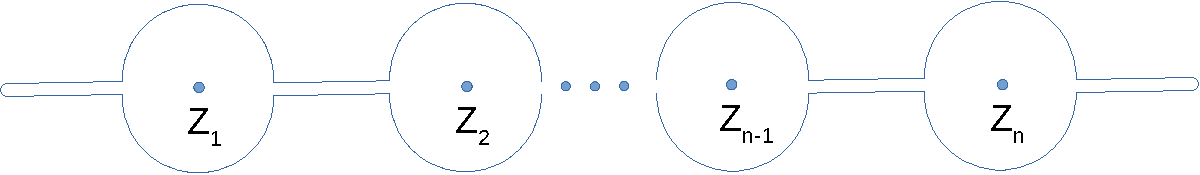
\includegraphics[scale=0.4]{images/lacet_compact.pdf}
    \caption{Lacet dans $X \setminus \cup_{i=1,\dots,n} \stackrel{\circ}{D_i}$}
    \label{fig:lacet_riemann_compact}
\end{figure}
\end{proof}

Un cas particulièrement important en pratique est celui de la sphère de Riemann, dont les application de changement de carte sont toutes deux $z \mapsto 1/z$. Si $f$ est une application méromorphe sur $\C$, elle définit une forme différentielle méromorphe de degré $1$ sur la carte identité et son expression dans la carte $z \mapsto 1/z$ est:
\[
g \colon z \neq 0 \mapsto \frac{-1}{z^2}f\left(\frac{1}{z}\right)
\]
En appliquant le théorème \ref{thm:residus_riemann}, on peut calculer une intégrale de contour en utilisant des points singuliers qui auraient été normalement à l'extérieur du lacet d'intégration. Le résidu en $0$ de l'application $g$ s'appelle résidu à l'infini. De façon générale, il est possible de passer d'une intégrale de contour dans $\C$ à une intégrale de contour dans $\overline{\C}$ en utilisant la transformation $z\mapsto 1/z$, ce qui inverse le sens de parcours du lacet. 
\section{Surfaces de Riemann concrètes}
Des cas similaires à la racine carrée se rencontrent fréquemment en pratique. Les surfaces de Riemann associées sont dites concrètes, car elles se réalisent sous la forme d'une partie de $\C^2$. 
\begin{defn}
Une surface de Riemann concrète est une partie $X \subset \C^2$ si elle peut être munie d'un système de cartes $(U_i,\phi_i)_{i \in I}$ tel que pour tout indice $i$, l'application réciproque $\phi_i^{-1}$ est de l'une des deux formes suivantes:
\[
\begin{cases}
\phi_i^{-1} \colon z \mapsto (z,f_i(z)) \\
\phi_i^{-1} \colon w \mapsto (g_i(w),w)
\end{cases}
\]
avec $f_i$ (resp. $g_i$) des applications holomorphes.
\end{defn}
Si deux cartes $(U_i,\phi_i),(U_j,\phi_j)$ sont telles que $\phi_i^{-1} \colon z \mapsto (z,f_i(z))$, $\phi_j^{-1} \colon w \mapsto (g_j(w),w)$, alors si $U_i \cap U_j \neq 0$, $f_i$ et $g_j$ sont inverses l'une de l'autre sur la partie commune. Ceci donne un procédé pratique de détermination de cartes locales de proche en proche en utilisant le principe du prolongement analytique. 

Les formes différentielles de degré $1$ sur une surface de Riemann concrète $X$ sont faciles à déterminer en utilisant la définition \ref{def:forme_degre_un}. Si l'on connaît l'expression d'une forme $\omega_i, i \in I$ dans une carte $(U_i,\phi_i)$ telle que $\phi_i^{-1} \colon z \mapsto (z,f_i(z))$ et que l'on souhaite l'exprimer sur le domaine commun avec une carte $(U_j,\phi_j)$ telle que $\phi_j^{-1} \colon w \mapsto (g_j(w),w)$, on aura:
\[
\omega_j(w) = \omega_i(z(w)) \partial_z z(w) \omega_i(z(w))
\]
avec $z(w) = \phi_i \circ \phi_j^{-1}(w)$
De façon symétrique, on passera d'une carte en $w$ à une carte en $z$ en posant:
\[
\omega_j(z) = \omega_i(w(z)) \partial_w w(z) \omega_i(w(z))
\]
avec $w(z) = \phi_i \circ \phi_j^{-1}(z)$.
\begin{rem}
Bien qu'elles soient appelées concrètes, les surfaces de Riemann associées à des fonctions usuelles ne sont pas nécessairement simples à déterminer. Il convient de garder à l'esprit qu'il s'agit avant tout d'un changement de variable et qu'il n'a donc d'intérêt que s'il est possible d'exprimer simplement la fonction à intégrer à l'aide de celle servant à construire la surface de Riemann.
\end{rem}
\section{Construction par coupure et recollement}
Une autre approche, plus géométrique et souvent plus facile à interpréter, consiste à partir d'autant de sphères de Riemann qu'il y a de déterminations possible de la fonction à représenter, puis à les recoller le long des coupures choisies. Le cas de l'application $z \mapsto \sqrt{1-z^2}$ servira à illustrer le procédé général. S'agissant d'une application faisant intervenir la racine carrée, qui possède deux déterminations, on partira donc de deux sphères de Riemann. Plusieurs coupures sont possibles, mais la plus simple en considérant les deux complexes $1-z,1+z$ dont les angles polaires, notés respectivement $\theta_1,\theta_2$ appartiennent aux intervalles $]-\pi,\pi[$  et $]0,2\pi[$ (voir figure \ref{fig:cut_angles}).
\begin{figure}[ht]
    \centering
    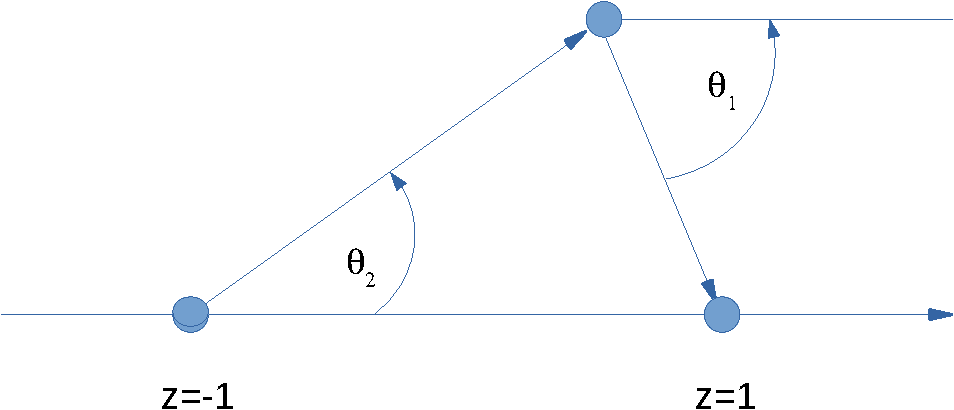
\includegraphics[scale=0.6]{images/riemann_exemple.pdf}
    \caption{Angles pour la détermination de la coupure}
    \label{fig:cut_angles}
\end{figure}
avec cette convention, il est possible d'obtenir une détermination continue de $z \mapsto \sqrt{1-z^2}$ sur $\C \setminus [-1,+1]$ en posant:
\[
\sqrt{1-z^2}=\sqrt{|1-z^2|}e^{i \theta_1/2}e^{i \theta_2/2}
\]
On remarque en effet que le franchissement du segment $]1,+\infty[$ implique deux changements de signe qui vont se compenser. La construction de la surface de Riemann de $z \mapsto \sqrt{1-z^2}$ se fera à partir de deux sphères coupées $\overline{\C} \setminus [-1,+1]$, dont les bords des coupures seront identifiés selon la figure  \ref{fig:gluing_spheres}.
\begin{figure}[ht]
    \centering
    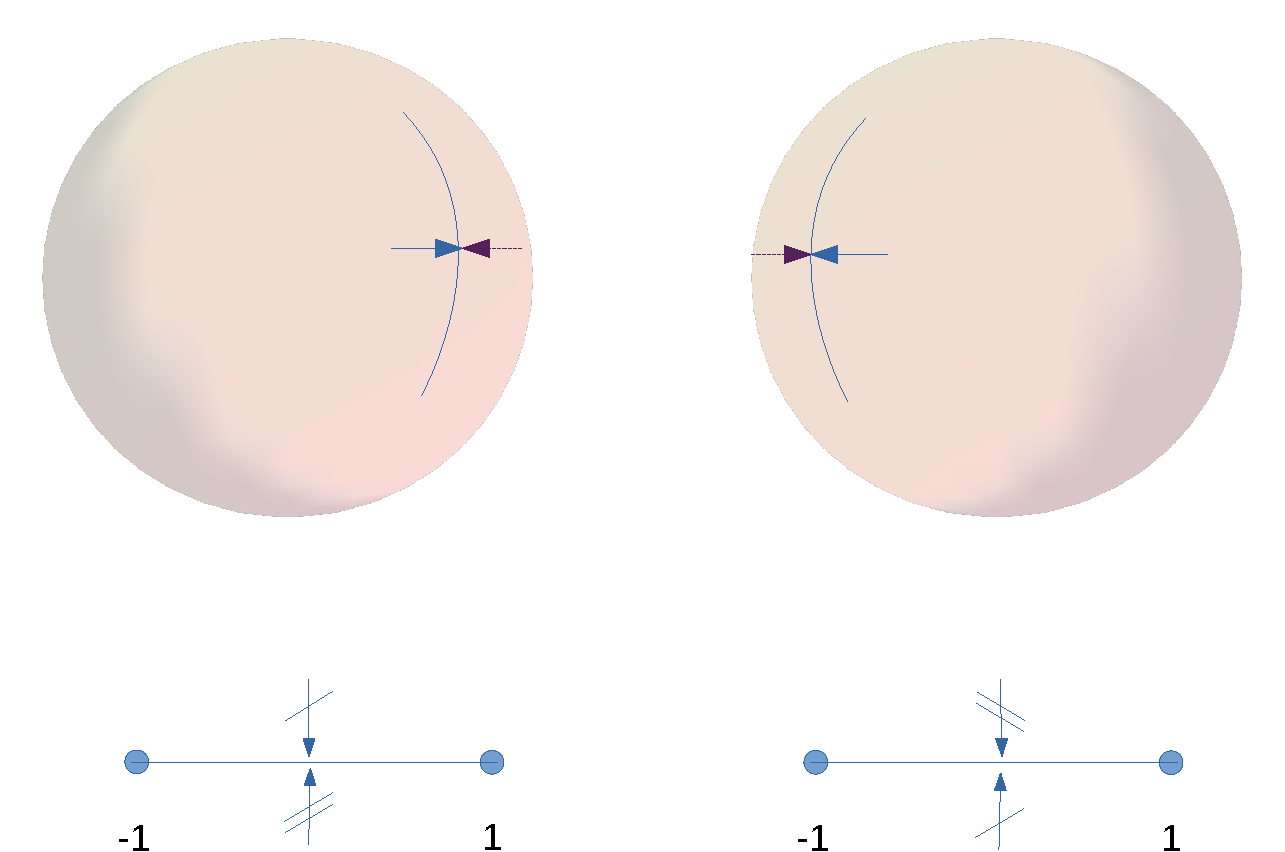
\includegraphics[scale=0.6]{images/recollement_spheres.pdf}
    \caption{Construction par recollement}
    \label{fig:gluing_spheres}
\end{figure}
L'objet obtenu est homémorphe à une sphère dont l'équateur est la coupure et les pôles les points à l'infini des sphères de Riemann d'origine. 
\begin{figure}[h!]
    \centering
    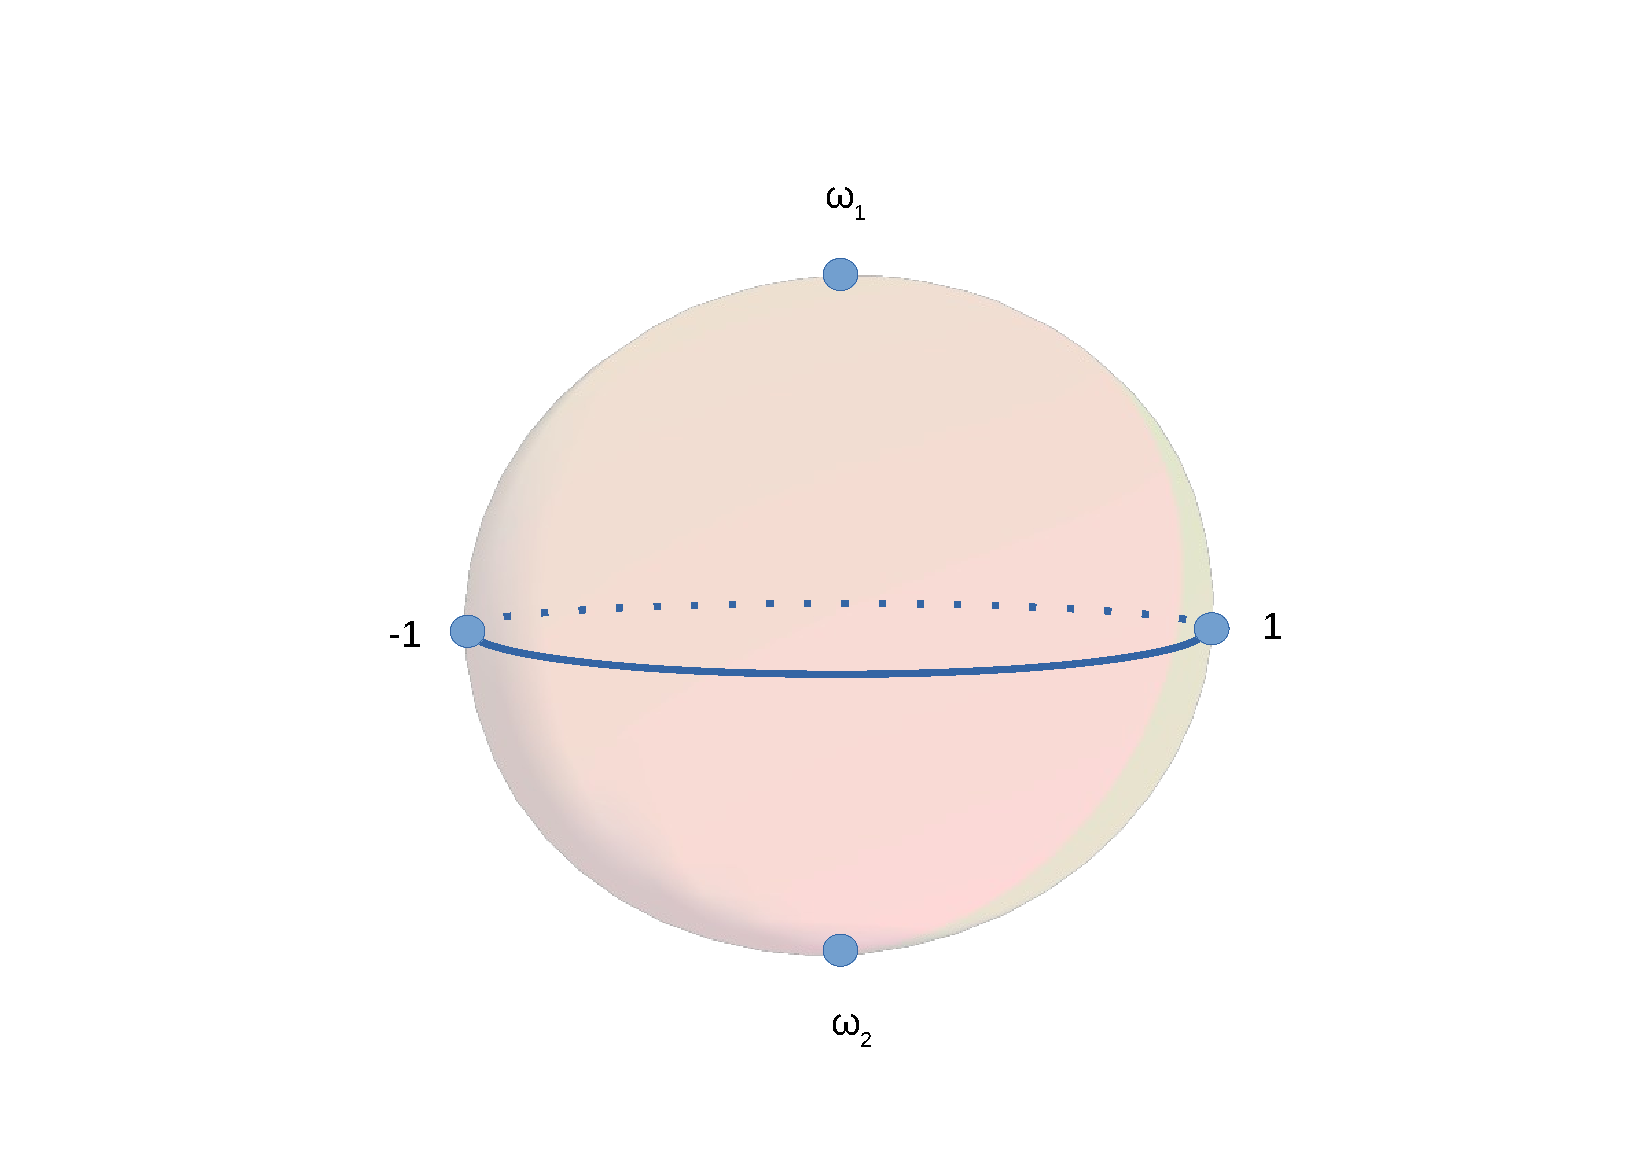
\includegraphics[scale=0.4]{images/surface_racine.pdf}
    \caption{Surface de $\sqrt{1-z^2}$}
    \label{fig:surface_racine_carre}
\end{figure}
On vérifie immédiatement que la détermination continue 
Les cas plus complexes conduisent à d'autres types de surface comme le montre l'exercice ci-dessous.
\begin{exercice}
Déterminer la surface de Riemann de $z \mapsto \sqrt{(1-z^2)(4-z^2)}$.
\leftline{Indication: On doit obtenir un tore de révolution.}
\end{exercice}
Le théorème des résidus sur les surfaces de Riemann permet de calculer des intégrales faisant intervenir des fonctions telles que la racine carrée. A partir de la construction précédente, on peut en particulier résoudre l'exercice suivant.
\begin{exercice}
Soit $a \in ]0,1[$. Déterminer la valeur de l'intégrale:
\[
\int_{-1}^1 \frac{1}{\sqrt{1-x^2}(1+ax)} dx
\]
\end{exercice}
\leftline{Elements de correction:}
La fonction de la variable complexe que l'on souhaite intégrer sera:
\[
f \colon z \mapsto \frac{1}{\sqrt{1-z^2}(1+az)}
\]
En raison de la présence au dénominateur de $\sqrt{1-z^2}$, on se placera sur la surface de Riemann de cette fonction. Il existe trois points singuliers: $z=-1, z=+1, z=-1/a$. Le contour d'intégration doit les éviter, on choisira celui présenté en figure \ref{fig:contour_riemann}, tel que lu dans une carte locale de la forme $(z,\sqrt{1-z^2})$
\begin{figure}[h!]
    \centering
    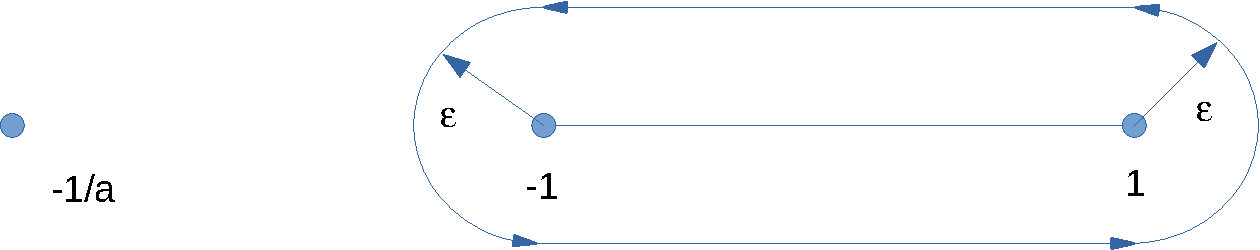
\includegraphics[scale=0.4]{images/contour_riemann.pdf}
    \caption{Contour d'intégration}
    \label{fig:contour_riemann}
\end{figure}
Lorsque $\epsilon$ tend vers $0^+$, la majoration ML montre que l'intégrale sur les arcs de cercles tend vers 0, alors qu'elle tend vers:
\[
\pm \int_{-1}^1 \frac{1}{\sqrt{1-x^2}(1+ax)} dx
\]
sur les deux branches horizontales. Au total, l'intégrale sur le long
du chemin tend vers:
\[
2 \int_{-1}^1 \frac{1}{\sqrt{1-x^2}(1+ax)} dx
\]
lorsque $\epsilon$ tend vers $0^+$.
En gardant le contour d'intégration sous l'équateur de la surface de Riemann de $\sqrt{1-z^2}$, on peut utiliser le théorème des résidus dans la demi-sphère. L'indice du point $z=-1/a$ par rapport au lacet n'est pas nul. En effet, l'intégrale :
\[
\frac{1}{i2\pi}\int_{\gamma}\frac{dz}{z+1/a} 
\]
doit se calculer en faisant intervenir le résidu à l'infini qui est le résidu en 0 de:
\[
\frac{-1}{z^2}\frac{1}{1/z +1/a} = \frac{-1}{z}\frac{1}{1+z/a}
\]
qui vaut $-1$.
Le lacet $\gamma$ étant parcouru en sens inverse trigonométrique après le changement de variable $z \mapsto 1/z$, on obtient finalement un indice de 1. 
Le résidu en $z=-1/a$ de l'application à intégrer vaut:
\[
\lim_{z \to -1/a} \frac{(z+1/a)}{\sqrt{1-z^2}(1+az)}
\]
soit:
\[
\frac{1}{a}\frac{1}{\sqrt{1-1/a^2}} = \frac{1}{\sqrt{a^2-1}} = \frac{1}{i\sqrt{1-a^2}} 
\]
Finalement, on doit calculer le résidu à l'infini, soit celui en 0 de:
\[
\frac{-1}{z^2}\frac{\sqrt{1-1/z^2}(1+a/z)} = \frac{-1}{\sqrt{z^2-1}(z+a)}
\]
qui est nul, l'application étant continue en $z = 0$.
En regroupant les termes, on obtient finalement que:
\[
2 \int_{-1}^1 \frac{1}{\sqrt{1-x^2}(1+ax)} dx = i 2 \pi \frac{1}{i\sqrt{1-a^2}}.
\]
Soit:
\[
\int_{-1}^1 \frac{1}{\sqrt{1-x^2}(1+ax)} dx = \frac{\pi}{\sqrt{1-a^2}}.
\]
On notera qu'il est possible de se limiter à une détermination (donc à une seule carte locale) en prenant un contour d'intégration tel que celui de la figure \ref{fig:contour_riemann_infty}. 
\begin{figure}[h!]
    \centering
    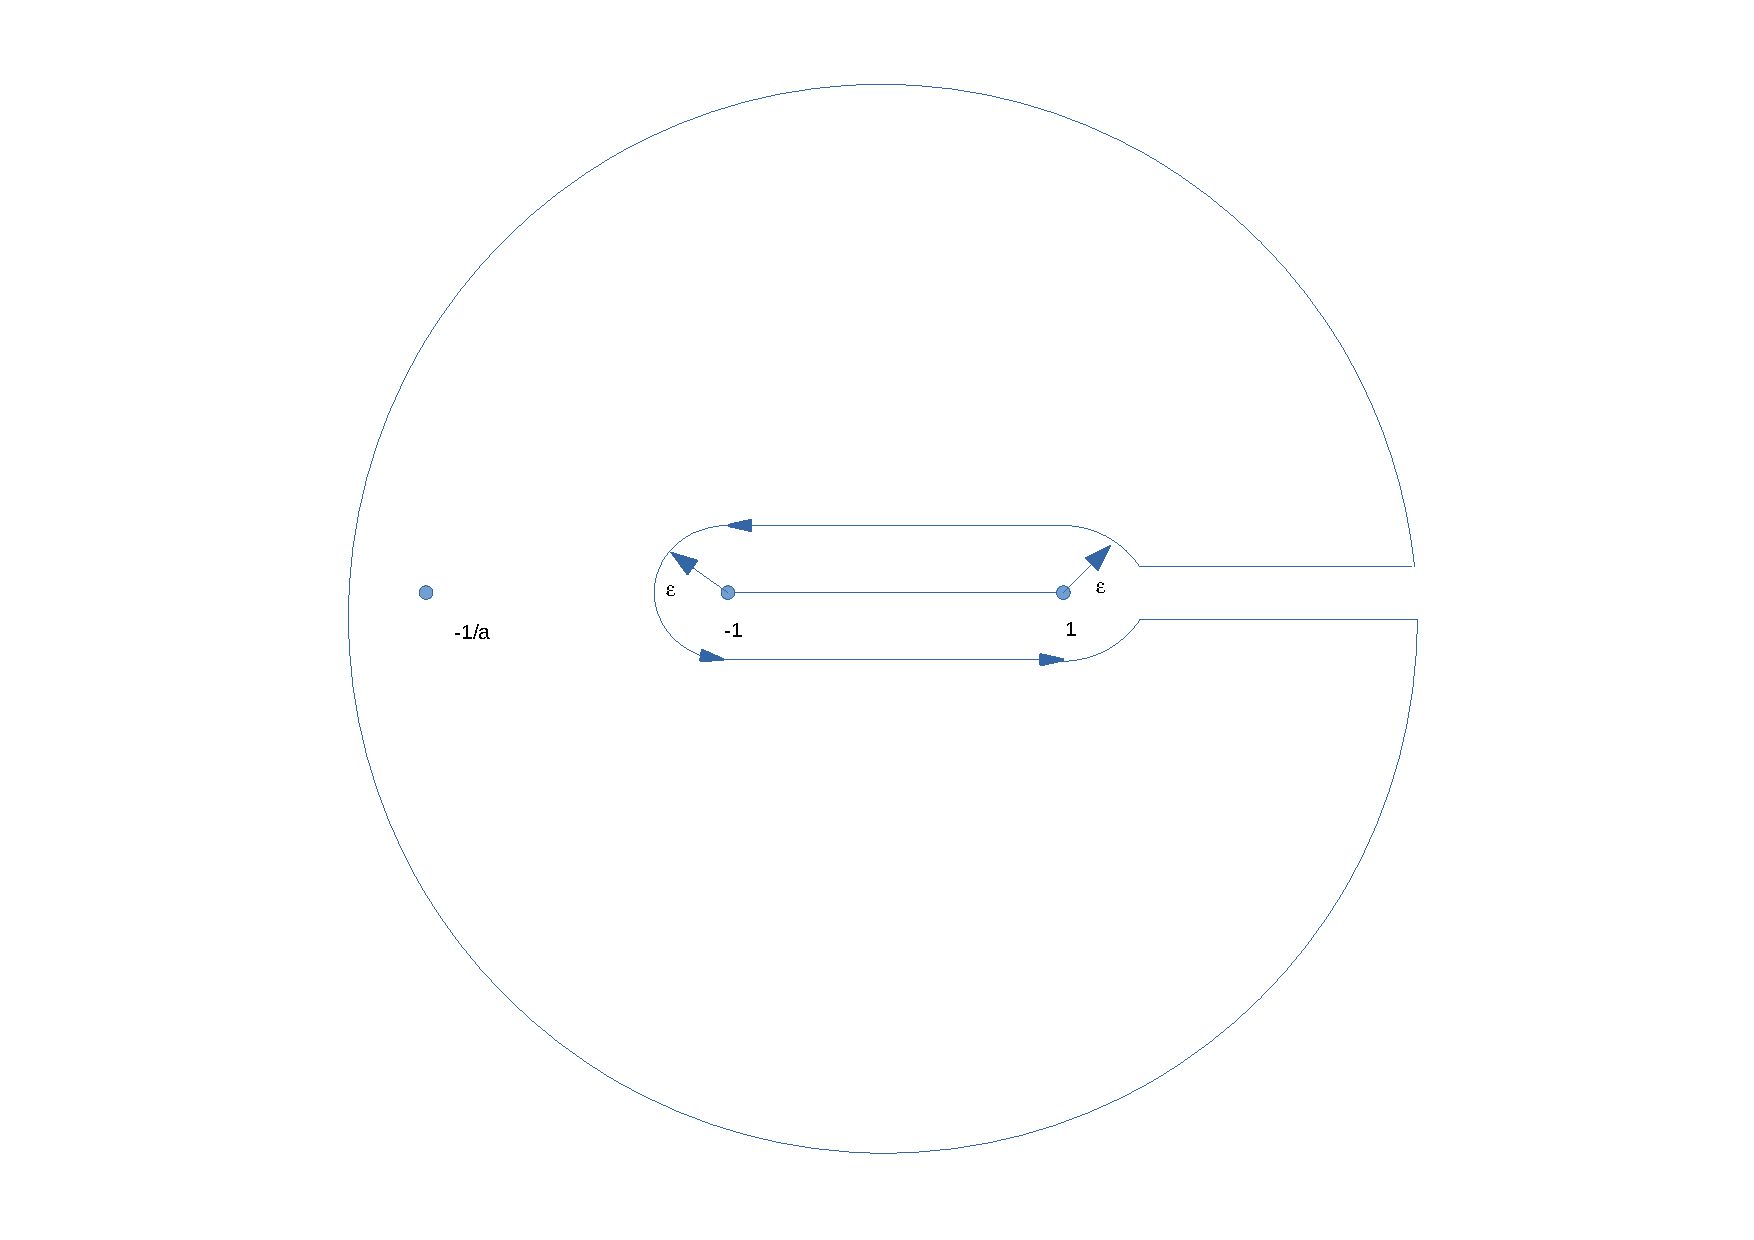
\includegraphics[scale=0.4]{images/contour_riemann_infty.pdf}
    \caption{Contour d'intégration}
    \label{fig:contour_riemann_infty}
\end{figure}
L'utilisation des surfaces de Riemann permet cependant d'éviter d'avoir à calculer la limite sur le cercle extérieur, qui sera précisément le résidu à l'infini.

\newpage 
\subsection*{Un peu d'histoire \dots}

\begin{minipage}{0.2\linewidth}
\begin{center}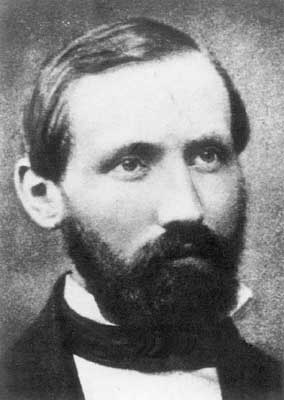
\includegraphics[width=2cm]{images/Riemann.jpg}\end{center}
\end{minipage}
\begin{minipage}{0.80 \linewidth}
\small{\paragraph*{Bernhard Riemann :} né le  17 Septembre 1826 à Breselenz (Basse-Saxe, Allemagne), mort le 20 Juillet 1866 à Semasca (Italie). Riemann est un des mathématiciens les plus importants de son époque et peut être de tous les temps. Durant sa courte carrière, il fonde la géométrie différentielle et contribue puissamment à l'étude des fonctions de la variable complexe. Il formalise la notion d'intégrale à partir de subdivisions de l'intervalle d'intégration.}
\end{minipage}

\vfill